\setchapterpreamble[u]{\margintoc}
\chapter{Wireless Network Security}
\labch{chapter6}

Fattori che rendono più rischiose le reti wireless rispetto a quelle cablate:
\begin{itemize}
    \item Canale: 
	\begin{itemize}
	    \item Le reti wireless in genere implicano comunicazioni broadcast, che sono molto più soggette a intercettazioni e disturbi rispetto alle reti cablate;
		\item Le reti wireless sono anche più vulnerabili agli attacchi attivi che sfruttano le vulnerabilità nei protocolli di comunicazione (Jamming);
	\end{itemize}
	\item Mobilità:
	\begin{itemize}
	    \item I dispositivi wireless sono molto più portatili e mobili rispetto ai dispositivi collegati con cavo. La mobilità comporta una serie di rischi;
	\end{itemize}
	\item Risorse:
	\begin{itemize}
	    \item Alcuni dispositivi wireless, come smartphone e tablet, dispongono di sistemi operativi sofisticati ma memoria e risorse di elaborazione limitate con cui contrastare le minacce, inclusi DDoS e malware;
	\end{itemize}
	\item Accessibilità:
	\begin{itemize}
	    \item Alcuni dispositivi wireless, come sensori e robot, potrebbero essere lasciati incustoditi in luoghi remoti e/o ostili, rendendoli più deboli ad attacchi fisici.
	\end{itemize}
\end{itemize}

\begin{figure}[h]
    \centering
    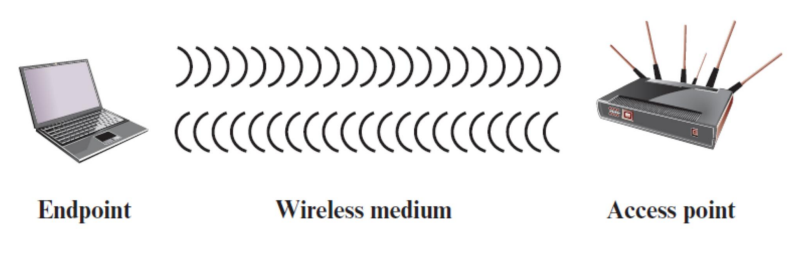
\includegraphics[width=1\textwidth]{images/chapter6/6-1.png}
    \caption{Reti wireless.}
    \label{fig:6-1}
\end{figure}

Minacce alle reti wireless:
\begin{itemize}
    \item Associazione accidentale: 
	\begin{itemize}
	    \item Wireless LAN aziendali create vicine tra loro potrebbero creare dei campi di trasmissione sovrapposti;
		\item Un utente che intende connettersi a una LAN potrebbe bloccarsi involontariamente su un punto di accesso wireless da una rete vicina;
	\end{itemize}
	\item Associazione dannosa: un dispositivo wireless è configurato per apparire come un access point legittimo, consentendo all'operatore di rubare le password di utenti legittimi e quindi penetrare in una rete cablata attraverso un punto di accesso wireless legittimo;
	\item Reti ad-hoc: si tratta di reti peer-to-peer tra computer wireless senza punti di accesso tra di loro. Possono rappresentare una minaccia per la sicurezza a causa della mancanza di un punto centrale di controllo;
	\item Reti non tradizionali: reti e collegamenti non tradizionali, come dispositivi Bluetooth di rete personale, lettori di codici a barre e palmari, rappresentano un rischio per la sicurezza sia in termini di intercettazione che di spoofing;
	\item MAC spoofing (furto di identità): si verifica quando un utente malintenzionato è in grado di intercettare il traffico di rete e identificare l'indirizzo MAC di un computer con privilegi di rete;
	\item Attacchi man-in-the-middle: questo attacco consiste nel persuadere un utente e un punto di accesso a credere che stiano parlando tra loro quando in realtà la comunicazione sta attraversando un dispositivo di attacco intermedio. Le reti wireless sono particolarmente deboli a questi attacchi;
	\item DDoS: questo attacco si verifica quando un utente malintenzionato bombarda continuamente un punto di accesso wireless o qualche altra porta wireless accessibile con vari messaggi di protocollo progettati per consumare risorse di sistema. L'ambiente wireless si presta a questo tipo di attacco perché è facile per l'attaccante indirizzare più messaggi wireless verso il bersaglio;
	\item Network injection: prende di mira i punti di accesso wireless che sono esposti a traffico di rete non filtrato, come messaggi del protocollo di instradamento o messaggi di gestione della rete.
\end{itemize}
		
Protezione delle trasmissioni wireless:
\begin{itemize}
    \item Le principali minacce alla trasmissione wireless sono le intercettazioni, le alterazione o inserimento di messaggi e interruzioni;
	\item Per affrontare le intercettazioni, esistono due tipi di contromisure:
	\begin{enumerate}
	    \item Tecniche di occultamento del segnale:
		\begin{itemize}
		    \item Disattivare la trasmissione SSID dai punti di accesso wireless;
			\item Assegnare nomi criptici agli SSID;
			\item Ridurre la potenza del segnale al livello più basso che fornisce comunque la copertura richiesta;
			\item Piazzare i punti di accesso wireless all'interno dell'edificio, lontano da finestre e pareti esterne.
		\end{itemize}
		\item Cifratura:
		\begin{itemize}
		    \item È efficace contro le intercettazioni nella misura in cui le chiavi sono protette.
		\end{itemize}
	\end{enumerate}
\end{itemize}

Protezione dei punti di accesso:
\begin{itemize}
    \item La principale minaccia che coinvolge i punti di accesso wireless è l'accesso non autorizzato alla rete;
	\item L'approccio principale per impedire tale accesso è lo standard IEEE 802.1x per il controllo dell'accesso alla rete basato su porte. L'uso di 802.1X può impedire che punti di accesso non autorizzati e altri dispositivi non autorizzati diventino backdoor non sicuri.
\end{itemize}

Raccomandazioni per la protezione delle reti wireless:
\begin{itemize}
    \item Usare la crittografia;
	\item Utilizzare software antivirus, antispyware e firewall;
	\item Disattivare la trasmissione broadcast dell'identificatore;
	\item Modificare l'identificatore sul router rispetto a quello predefinito;
	\item Modificare la password preimpostata del router;
	\item Consenti solo a computer specifici di accedere alla rete wireless.
\end{itemize}

\section{Sicurezza dei dispositivi mobili}

I dispositivi mobili sono diventati un elemento essenziale per le organizzazioni come parte dell'infrastruttura di rete complessiva. Prima dell'uso diffuso degli smartphone, la sicurezza della rete si basava su perimetri chiaramente definiti che separavano le reti interne affidabili da Internet. A causa di enormi cambiamenti, le reti di un'organizzazione devono ora ospitare: un uso crescente di dispositivi, applicazioni cloud, deperimetrizzazione, requisiti aziendali esterni (ospiti in visita).

Problemi principali per la sicurezza dei dispositivi mobili:
\begin{itemize}
    \item Utilizzo di app create da sconosciuti: è facile trovare e installare applicazioni di terze parti sui dispositivi mobili e ciò comporta il rischio di installare software dannoso;
	\item Interazione con altri sistemi: a meno che un'organizzazione non abbia il controllo di tutti i dispositivi coinvolti nella sincronizzazione, esiste un rischio considerevole che i dati dell'organizzazione vengano archiviati in una posizione non protetta, oltre al rischio di introduzione di malware;
	\item Utilizzo dei servizi di localizzazione: un utente malintenzionato può utilizzare le informazioni sulla posizione per determinare dove si trovano il dispositivo e l'utente.
\end{itemize}

\paragraph{Policy bring-your-own-device} Se l'utente può portare a casa il dispositivo aziendale, è necessario che l'azienda implementi una forte policy di sicurezza, per evitare che il dispositivo o la rete, quando il dispositivi viene ricollegato, vengano attaccati. Implemento quindi una:
\begin{itemize}
    \item Sicurezza nel dispositivi: blocco automatico, antivirus, PIN;
	\item Sicurezza nel traffico della rete: TLS, autenticazione forte, VPN;
	\item Barriere all'ingresso della rete: firewall, IDS.
\end{itemize}

\section{Standard IEEE 802.11}

IEEE 802 è un comitato che ha sviluppato standard per un'ampia gamma di reti locali (LAN). Nel 1990 il Comitato IEEE 802 ha formato un nuovo gruppo di lavoro, IEEE 802.11, per sviluppare un protocollo e specifiche di trasmissione per LAN wireless (WLAN). 

Definizioni:
\begin{enumerate}
    \item Access Point (AP): qualsiasi entità che dispone della funzionalità della stazione e fornisce l'accesso al sistema tramite il supporto wireless per le stazioni associate;
	\item Basic Service Set (BSS): insieme di stazioni controllate da un'unica coordination function;
	\item Coordination Function: funzione logica che determina quando una stazione operante all'interno di un BSS è autorizzata a trasmettere e può essere in grado di ricevere PDU;
	\item Distribution System (DS): sistema utilizzato per interconnettere un insieme di BSS e LAN integrate per creare un ESS;
	\item Extended Service Set (ESS): insieme di uno o più BSS interconnessi e LAN integrate che appaiono come un singolo BSS al livello LLC in qualsiasi stazione associata a uno di questi BSS;
	\item MAC protocol data unit (MPDU): unità di dati scambiati tra due entità MAC peer utilizzando i servizi del livello fisico;
	\item MAC service data unit (MSDU): informazioni consegnate come unità tra utenti MAC;
	\item Stazione: Qualsiasi dispositivo che contenga un MAC e un layer fisico conforme a IEEE 802.11.
\end{enumerate}

\subsection{Stack del protocollo IEEE 802.11}

\begin{figure}[h]
    \centering
    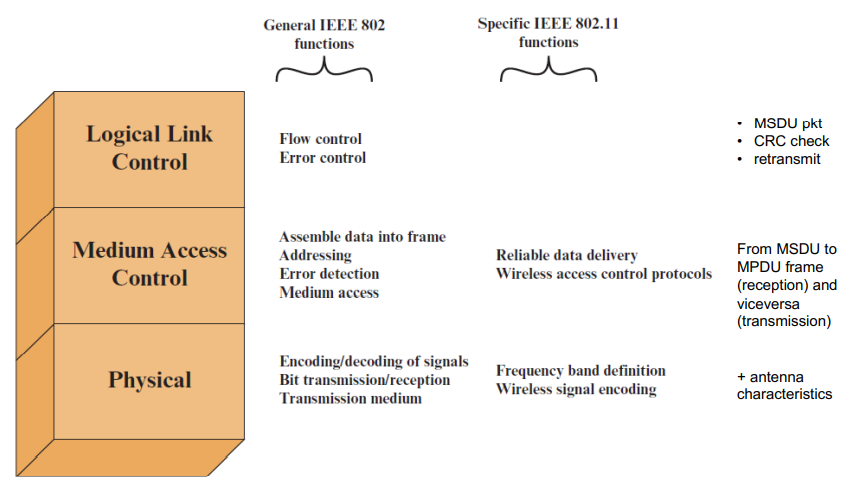
\includegraphics[width=1\textwidth]{images/chapter6/6-2.png}
    \caption{Stack del protocollo IEEE 802.11.}
    \label{fig:6-2}
\end{figure}

\begin{itemize}
    \item Logical link control:
	\begin{itemize}
	    \item 802 -> controllo del flusso, controllo degli errori;
	\end{itemize}
	\item Medium Access Control:
	\begin{itemize}
	    \item 802 -> assembra i dati in frame, indirizzamento, individuazione degli errori, accesso al medium;
		\item 802.11 -> consegna affidabile, protocolli di access control wireless;
	\end{itemize}
	\item Layer fisico:
	\begin{itemize}
	    \item 802 -> encoding/decoding del segnale, trasmissione/ricezione dei bit;
		\item 802.11 -> definizione della frequenza della banda, encoding del segnale wireless.
	\end{itemize}
\end{itemize}

\subsection{Formato MPDU in IEEE 802}

\begin{figure}[h]
    \centering
    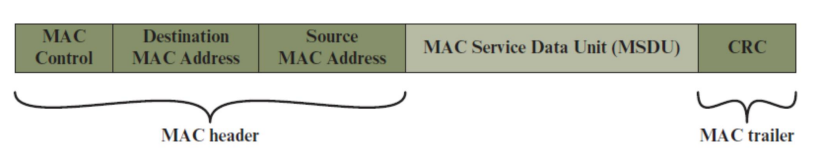
\includegraphics[width=1\textwidth]{images/chapter6/6-3.png}
    \caption{Formato MPDU in IEEE 802.}
    \label{fig:6-3}
\end{figure}

Campi:
\begin{itemize}
    \item MAC control: info di controllo del protocollo come livello di priorità;
	\item Indirizzo MAC di destinazione: indirizzo fisico di destinazione sulla LAN;
	\item Indirizzo MAC di origine: indirizzo fisico di origine sulla LAN;
	\item MSDU: dati dal livello successivo superiore;
	\item CRC (Cyclic redundancy check): ridondanza ciclica, campo di controllo sui bit dell'intera MDPU.
\end{itemize}

\subsection{IEEE 802.11 Extended Service Set (EES)} 

\begin{figure}[h]
    \centering
    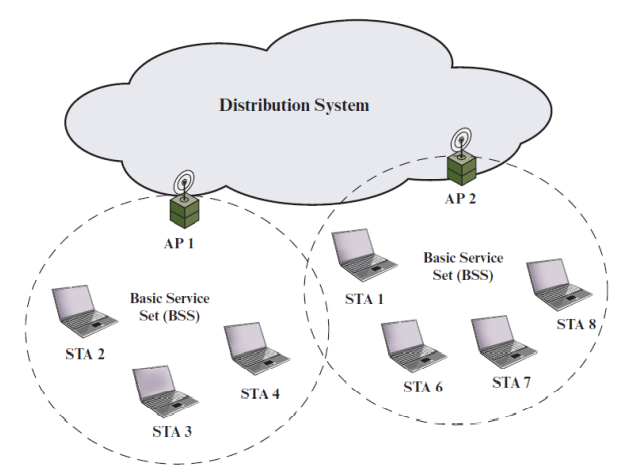
\includegraphics[width=1\textwidth]{images/chapter6/6-4.png}
    \caption{IEEE 802.11 Extended Service Set (EES).}
    \label{fig:6-4}
\end{figure}

\subsection{Servizi IEEE 802.11}

I servizi per la distribuzione dei messaggi all'interno del DS sono:
\begin{itemize}
    \item Distribution: servizio principale utilizzato dalle stazioni per lo scambio MPDU quando le MPDU devono attraversare il DS per andare da una stazione in un BSS a una stazione in un altro BSS;
	\item Integration: consente il trasferimento di dati tra una stazione su una LAN IEEE 802.11 e una stazione su una LAN IEEE 802.x integrata (cablata). Si occupa di ogni traduzione degli indirizzi e delle logiche di conversione dei media necessarie per lo scambio dei dati.
\end{itemize}

Per quanto riguarda i servizi relativi all'associazione, lo standard definisce 3 tipi di transizioni:
\begin{itemize}
    \item Nessuna transizione: la stazione è fissa o si muove solo all'interno del raggio di comunicazione diretta delle stazioni comunicanti di un singolo BSS;
	\item Transizione BSS: movimento della stazione da un BSS a un altro BSS all'interno dello stesso ESS. La consegna dei dati alla stazione richiede che la capacità di indirizzamento sia in grado di riconoscere la nuova posizione della stazione;
	\item Transizione ESS: spostamento della stazione da un BSS in un ESS a un BSS all'interno di un altro ESS. È probabile che si verifichi un'interruzione del servizio.
\end{itemize}

Per recapitare un messaggio all'interno di un DS, il servizio di distribuzione deve conoscere l'identità dell'AP a cui deve essere consegnato il messaggio affinché il messaggio raggiunga la stazione di destinazione. 
I servizi che si occupano di mantenere l'associazione della stazione all'Access Point all'interno del BSS corrente sono:
\begin{itemize}
    \item Associazione: stabilisce un'associazione iniziale tra stazione e AP;
	\item Riassociazione: permette di trasferire un'associazione già stabilita da un AP ad un altro, permettendo ad una stazione di passare da un BSS a un altro;
	\item Disassociazione: notifica da parte della stazione o dell'AP che l'associazione esistente è terminata.
\end{itemize}

\subsection{Sicurezza delle WLAN - IEEE 802.11i}

I servizi di protezione delle WLAN adottati sono:
\begin{itemize}
    \item Wired Equivalent Privacy (WEP): porzione relativa alla privacy dello standard IEEE 802.11. Conteneva gravi debolezze;
	\item Wi-Fi Protected Access (WAP): insieme di meccanismi di sicurezza che elimina la maggior parte dei problemi di sicurezza 802.11. Basato sullo stato attuale dello standard 802.11i;
	\item Robust Network Security (RNS o WAP2/WAP3): forma finale dello standard IEEE 802.11i 2012. Molto complesso. Garantisce:
	\begin{itemize}
	    \item Access Control;
		\item Autenticazione e generazione delle chiavi;
		\item Confidenzialità, autenticazione dell'origine dei dati, integrità e protezione dai replay attack.
	\end{itemize}
\end{itemize}

Fasi operative della sicurezza stazione-Access Point
\begin{enumerate}
    \item \textbf{Discovery}: l'AP invia messaggi beacon per dire che esiste. La stazione che vuole collegarsi risponde e si associa, scegliendo, tra le proposte inserite nel beacon, il cypher suite e il meccanismo di autenticazione da usare;
	\item \textbf{Authentication}: durante questa fase, la STA e l'Authentication Server si identificano reciprocamente. l'AP blocca il traffico di non autenticazione tra STA e AS finché l'autenticazione non riesce .L'unica cosa che fa AP in questa fase è inoltrare traffico tra STA e AS;
	\item \textbf{Key management}: l'AP e la STA eseguono diverse operazioni che determinano la generazione e il posizionamento di chiavi crittografiche sull'AP e sulla STA. I frame vengono scambiati solo tra AP e STA;
	\item \textbf{Protected Data Transfer}: i frame vengono scambiati tra la STA e la stazione finale tramite l'AP. Il trasferimento sicuro dei dati avviene solo tra la STA e l'AP (come indicato dall'ombreggiatura e dall'icona del modulo di crittografia); la sicurezza non è fornita end-to-end. Infatti le chiavi crittografiche se le sono scambiate la stazione e l'AP, quindi la comunicazione sarà STA -> AP, AP -> STA2;
	\item \textbf{Connection termination}: la connessione protetta viene interrotta e la connessione viene ripristinata allo stato originale.
\end{enumerate}

\begin{figure}[h]
    \centering
    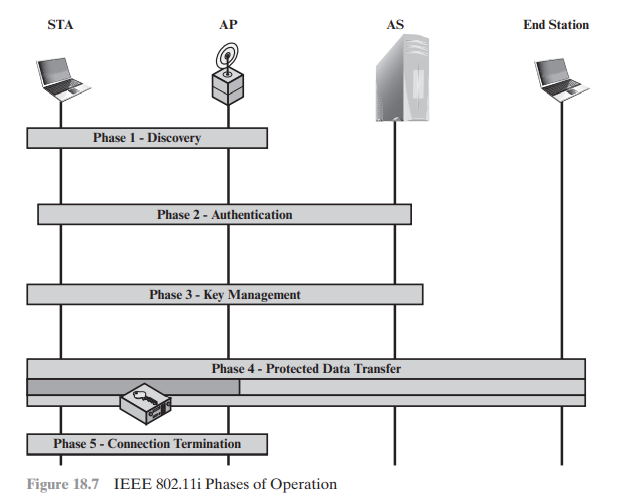
\includegraphics[width=1\textwidth]{images/chapter6/6-5.png}
    \caption{Fasi IEEE 802.11i.}
    \label{fig:6-4}
\end{figure}

Lo scopo di questa fase è che una STA e un AP si riconoscano, si accordino su una serie di capacità di sicurezza e stabiliscano un'associazione per la comunicazione futura utilizzando tali capacità di sicurezza. I passi di questa fase sono:
\begin{enumerate}
    \item \textbf{Probe request/response}: la STA risponde al beacon dell'AP, proponendosi alla connessione. L'AP trasmette periodicamente le proprie capacità di sicurezza in un canale specifico attraverso il Beacon. Le capacità di sicurezza non sono negoziabili, quindi se la STA non le accetta la connessione termina;
	\item \textbf{Open system authentication}: i due dispositivi (STA e AP) si scambiano semplicemente degli identificatori. Questo passo è necessario per garantire la compatibilità con le versioni precedenti di 802.11;
	\item \textbf{Association}: la STA invia un frame di richiesta di associazione all'AP. In questo passo, la STA specifica un insieme di funzionalità (autenticazione e gestione delle chiavi, crittografia) tra quelle pubblicizzate dall'AP. Se non c'è corrispondenza nelle capacità tra l'AP e la STA, l'AP rifiuta la richiesta di associazione;
\end{enumerate}

\begin{figure}[h]
    \centering
    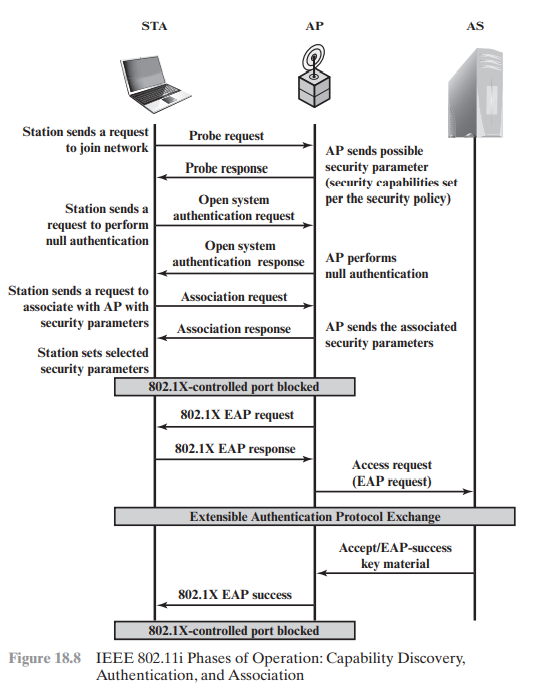
\includegraphics[width=1\textwidth]{images/chapter6/6-6.png}
    \caption{Fasi IEEE 802.11i (pt.2).}
    \label{fig:6-4}
\end{figure}

La fase di autenticazione consente l'autenticazione reciproca tra una STA e un server di autenticazione (AS) situato nel DS. L'autenticazione è progettata per consentire solo alle stazioni autorizzate di utilizzare la rete e per fornire alla STA la certezza che sta comunicando con una rete legittima. L'autenticazione viene effettuata tramite il protocollo EAP (Extensible Authentication Protocol).
L'AS si trova generalmetne len lato cablato della rete, anche se a volte può essere nell'AP.
L'AS genera una Master Session Key (MSK) e invia alla STA tramite EAP. Tutte le altre chiavi sono generate a partire dalla MSK.

A partire dalla master key, vengono generate una serie di chiavi, che possono essere divise in 2 tipologie:
\begin{itemize}
    \item Per comunicazioni simmetriche point to point da un dispositivo ad un altro (comunicazioni pairwise);
	\item Per comunicazioni di gruppo (broadcast, le chiavi sono comuni al gruppo).
\end{itemize}

Per il trasferimento protetto dei dati, IEEE 802.11i definisce due possivili schemi:
\begin{itemize}
    \item Tempora Key Integrity Protocol (TKIP): ora deprecato, è stato progettato per richiedere solo modifiche software ai dispositivi implementati con WEP. Fornisce due servizi:
	\begin{itemize}
	    \item Integrità del messaggio: aggiunge un codice di integrità del messaggio (MIC) al frame;
		\item Riservatezza dei dati: MPDU + MIC sono crittografati utilizzando RC4.
	\end{itemize}
	\item Counter Mode-CBC MAC Protocol (CCMP): destinato ai dispositivi IEEE 802.11 più recenti che sono dotati dell'hardware per supportarlo. Fornisce due servizi:
	\begin{itemize}
	    \item Integrità del messaggio: utilizza il MAC concatenamento di blocchi di crittografia;
		\item Riservatezza dei dati: utilizza la modalità di cifratura a blocchi CTR con AES.
	\end{itemize}
\end{itemize}

Per la generazione delle chiavi vengono usare pseudorandom function.
